\documentclass[a4paper,12pt]{extreport}
\usepackage[utf8]{inputenc}
\usepackage[russian]{babel}
\usepackage{ragged2e}
\usepackage[mag=1000,a4paper,left=1cm,right=1cm,top=1cm,bottom=1cm,noheadfoot]{geometry}
\usepackage{mathtext}
\usepackage{amsmath,amssymb,amsthm,amscd,amsfonts,graphicx,epsfig,textcomp,wrapfig}
\usepackage[dvips]{graphicx}
\graphicspath{{noiseimages/}}

\newcommand{\tab}{\hspace{10mm}}
\newcommand{\name}{
			\normalsize
			{
				\ \ \quad
                \mbox{} \hfil {\flushleft{5 школа}} \hfill {12.03.2024}
			%\quad
			}
			\vspace{5pt}\hrule
		}

\def\head#1#2{
	\begin{center}{
			\LARGE
			\bf #2
			
			{\normalsize \bf #1}
			\vspace{-10pt}
	}\end{center}
}

\newcommand{\del}{\mathop{\raisebox{-2pt}{\vdots}}}
\newcommand{\q}{}

\newcounter{tasknum}
\setcounter{tasknum}{0}
\def\thetasknum{{\textbf{\arabic{tasknum}}}}
\newcommand{\task}{\refstepcounter{tasknum}\vspace{2pt}\noindent \textbf{} \thetasknum\textbf{.}~}
\newcommand{\coff}{\refstepcounter{tasknum}\vspace{2pt}\noindent \textbf{Задача} \thetasknum *\textbf{.}~}


\newcommand{\eq}[1]{\underset{#1}{\equiv}}
\newcommand{\dv}{\ensuremath{\mathop{\raisebox{-2pt}{\vdots}}}}
\newcommand{\ndv}{\not \dv}

\newcounter{exnum}
\setcounter{exnum}{0}
\def\theexnum{{\emph{\arabic{exnum}}}}
\newcommand{\ex}{\refstepcounter{exnum}\vspace{2pt}\noindent \emph{Упражнение} \theexnum\emph{.}~}



\theoremstyle{plain}
\newtheorem{theorem}{Теорема}
\newtheorem{lemma}{Лемма}
\newtheorem{proposition}{Предложение}
\newtheorem{corollary}{Следствие}
\theoremstyle{definition}
\newtheorem{definition}{Определение}
\theoremstyle{remark}
\newtheorem{remark}{Замечание}
\newtheorem{example}{Пример}

\textheight=250mm %
\textwidth=180mm %
\oddsidemargin=-10.4mm%
\evensidemargin=-10.4mm %
\topmargin=-24.4mm


\begin{document}
	\pagestyle{empty}
    \name{}
	\head{6 класс}{Умники и дороги.}
	\bigskip
	
\task В лагере собралось $6$ именинников и несколько неименинников. Каждый неименинник поздравил двоих именинников, при этом каждому имениннику досталось по три поздравления. Сколько неименинников?\\

\task Можно ли расставить числа $1, 2, \dots , 8, 9$ по кругу так, чтобы сумма никаких двух соседних чисел не делилась ни на $3$, ни на $5$, ни на $7$? \\

\task В стране Цифра есть $9$ городов с названиями $1, 2, 3, 4, 5, 6, 7, 8, 9$. Путешественник обнаружил, что два города соединены авиалинией в том и только в том случае, если двузначное число, составленное из цифр названий этих городов, делится на $3$. Назовите все города, в которые можно добраться из города $1$.\\
b. Та же задача, но города соединены, если из их номеров можно составить число, кратное $7$.\\
c. Та же задача,но теперь кратное $8$.
\\

\begin{wrapfigure}{r}{0.35\textwidth} 
  \vspace{-40pt}
  \begin{center}
  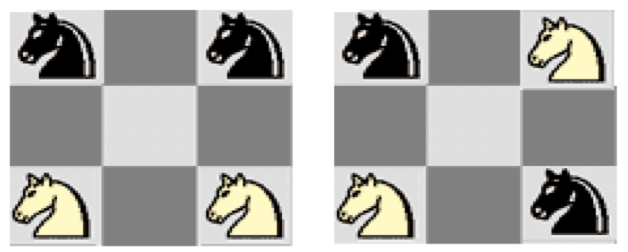
\includegraphics[width=0.35\textwidth]{pic_1.png} 
  \end{center}
\end{wrapfigure}

\task Кони стоят так, как показано на левом рисунке. Ходы происходят по шахматным правилам. Могут ли через несколько ходов кони встать так, как показано на правом рисунке?\\
\\

\begin{wrapfigure}{r}{0.15\textwidth} 
  \vspace{-45pt}
  \begin{center}
  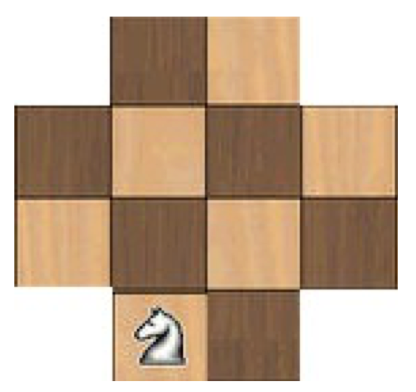
\includegraphics[width=0.15\textwidth]{pic_2.png} 
  \end{center}
\end{wrapfigure}

\task Доска имеет форму креста, который получается, если из квадратной доски $4 \times 4$ выкинуть угловые клетки. Можно ли обойти ее ходом шахматного коня и вернуться на исходное поле, побывав на всех полях ровно по разу?\\

\task В N-ском уезде Графландии уезде $20$ усадеб. И в этом уезде любые две дороги имеют общий конец. Докажите, что найдутся $18$ усадеб, никакие две из которых не
соединены дорогой.\\

\task В одной стране из каждого города выходит не более трёх дорог. При этом из каждого города можно добраться до любого другого не более чем с одной пересадкой. Каково наибольшее возможное число городов в этой стране? \\

\end{document}
